% !TEX root = ../main.tex

%-------------------------------------------------------------------------------
%-------------------------------------------------------------------------------
\begin{frame}\frametitle{Public outreach}

\centering
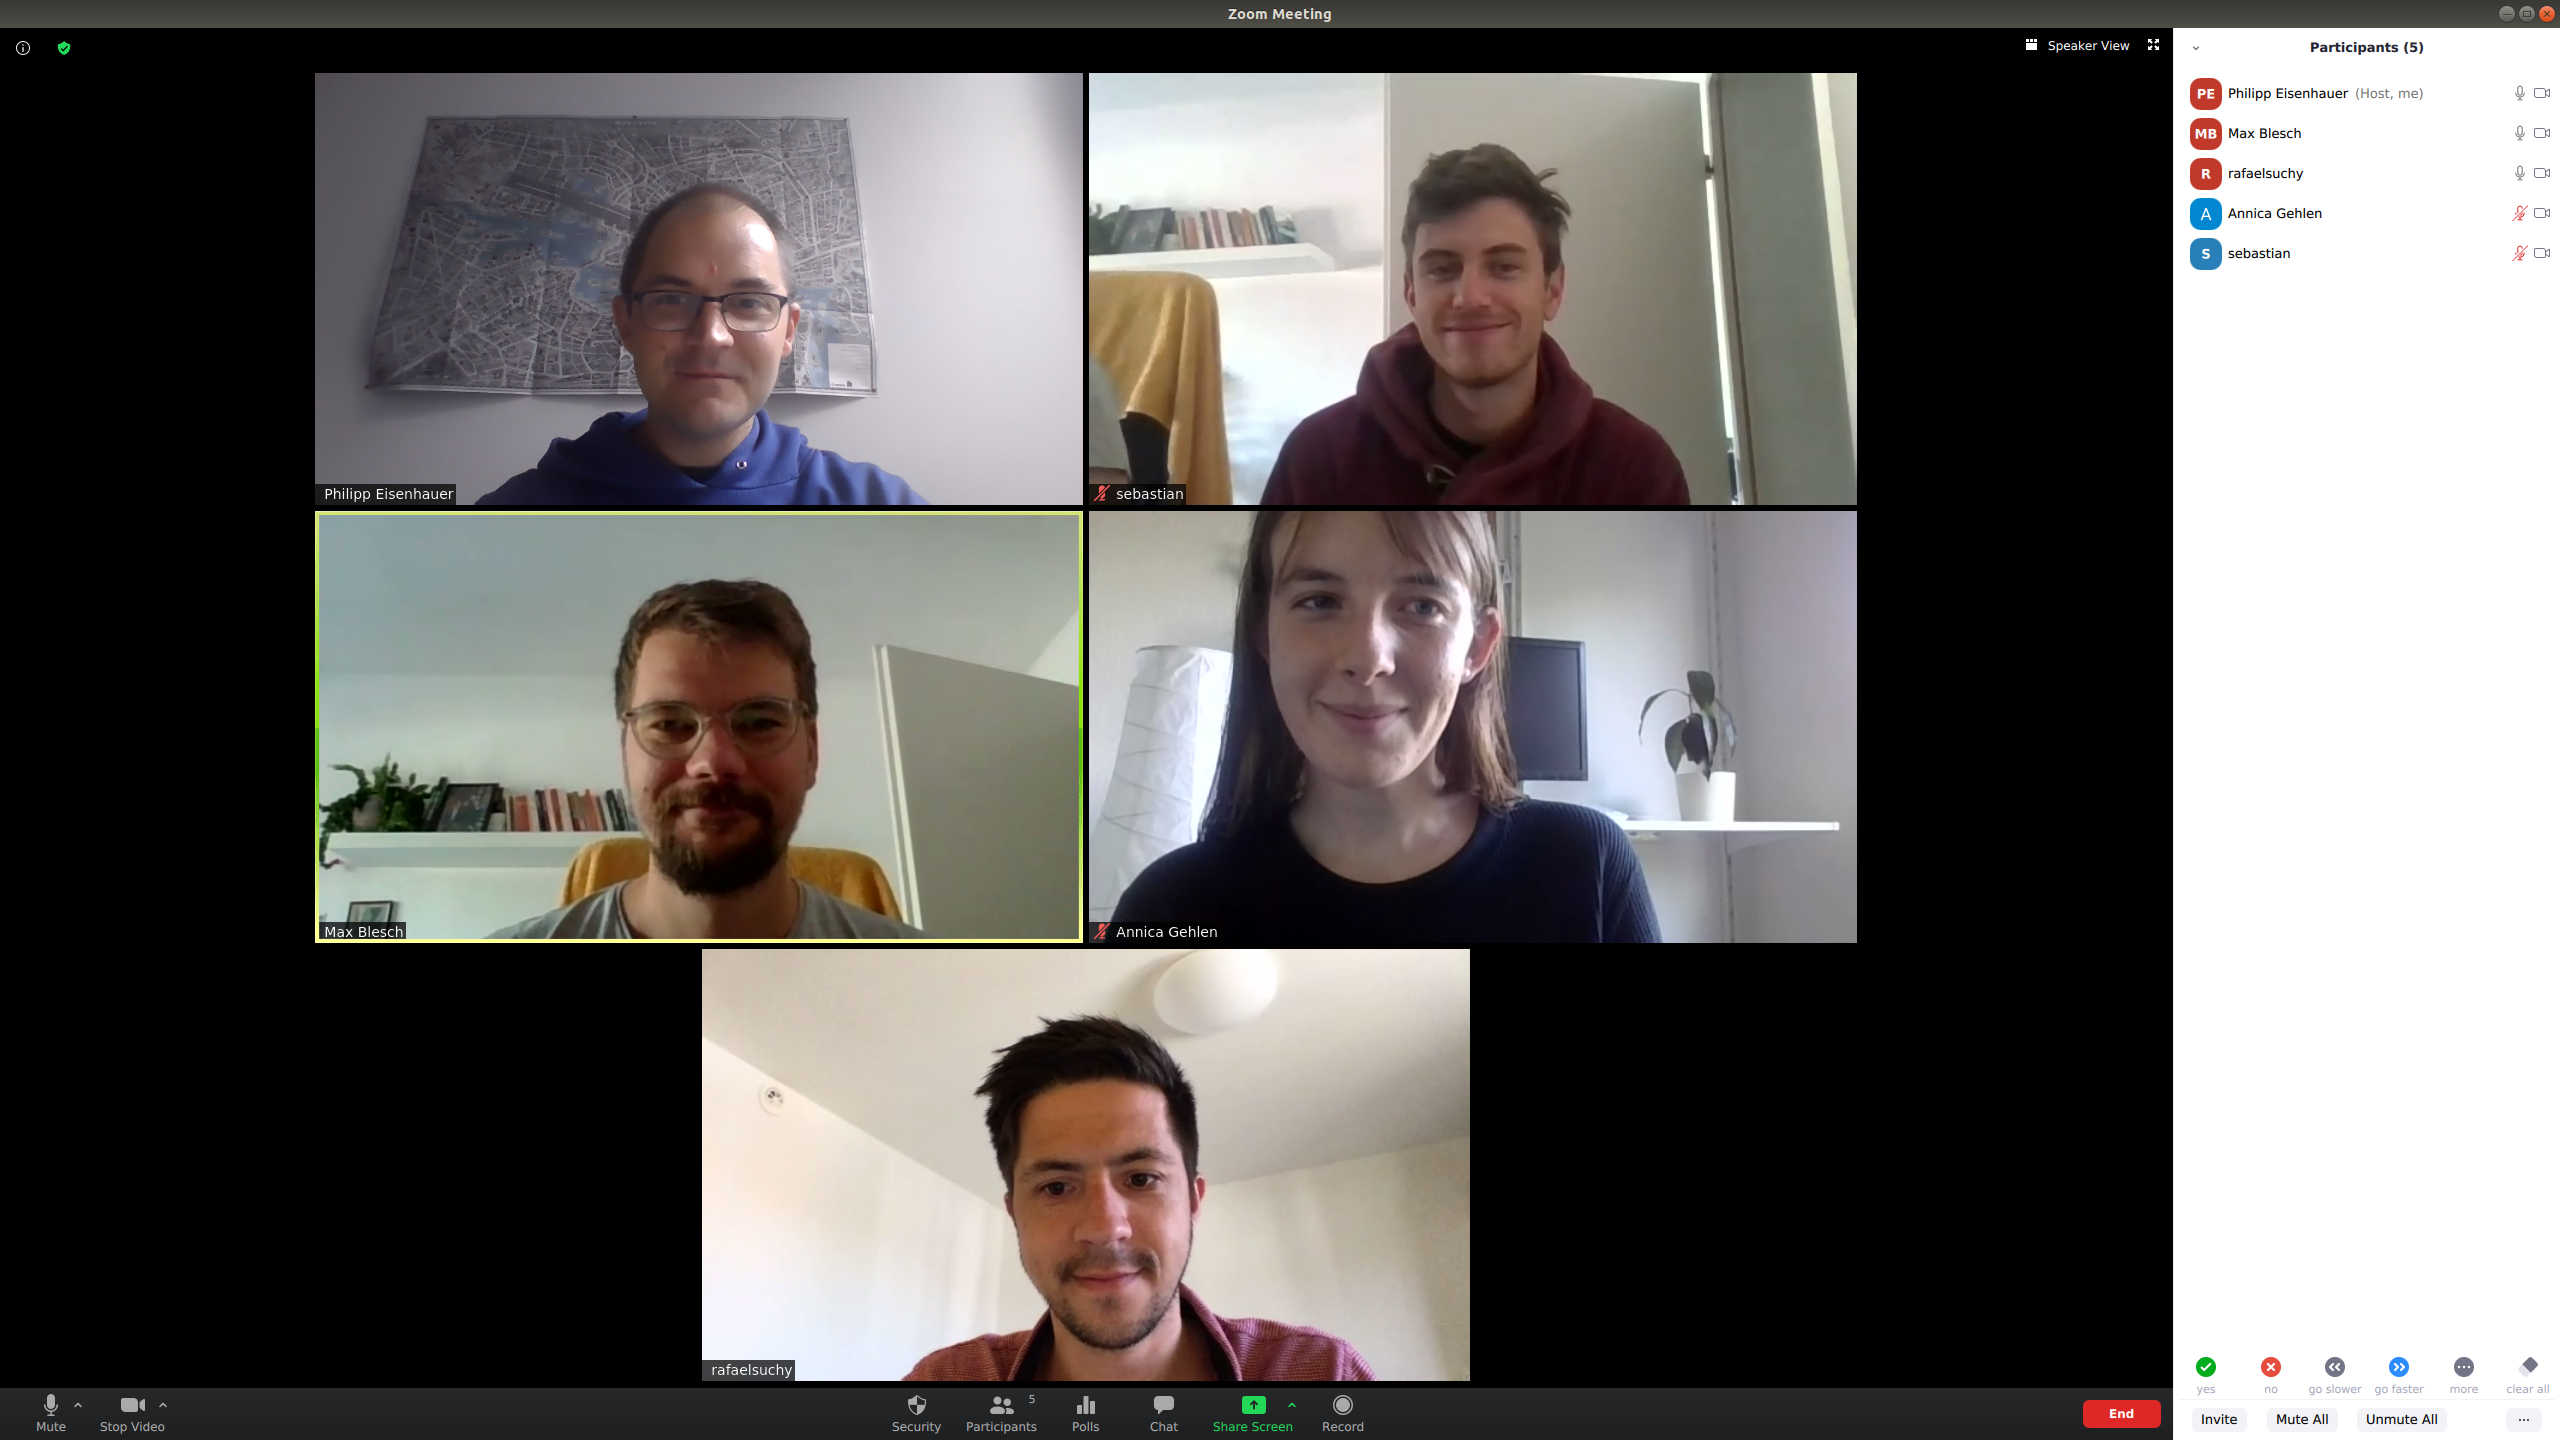
\includegraphics[width=0.52\textwidth]{material/crop-zoom-meeting.png}\\

\end{frame}

%-------------------------------------------------------------------------------
%-------------------------------------------------------------------------------
\begin{frame}\frametitle{In a nutshell}
\hspace{1.5cm}
\vspace{0.25cm}

\begin{quote}
	\large
	\raggedright
	\linespread{1.3}\selectfont{}
	We provide a platform for economists, mathematicians, and computational scientists to facilitate the \alert{transdisciplinary collaboration} in the development, analysis, and application of \alert{computational economic models}.
	\medskip \\
	Together, we \alert{expand the set} of possible economic questions that we can address and \alert{improve the quality} of our answers.
\end{quote}

\end{frame}

%-------------------------------------------------------------------------------
%-------------------------------------------------------------------------------
\begin{frame}\frametitle{Computational modeling in economics}

	\begin{multicols}{2}
	\heading{Motivation}\vspace{0.3cm}
	\begin{itemize}\setlength\itemsep{1em}
	\item Facilitate learning
	\item Study mechanisms
	\item Predict public policies
	\end{itemize}

	\pause

  \heading{Transdisciplinary in nature}\vspace{0.3cm}
	\begin{itemize}\setlength\itemsep{1em}
	\item Economic model
	\item Mathematical framework
	\item Computational implementation
	\end{itemize}
	\end{multicols}

\end{frame}

%-------------------------------------------------------------------------------
%-------------------------------------------------------------------------------
\begin{frame}\frametitle{New tooling for an old idea}

\vspace{0.3cm}
\centering
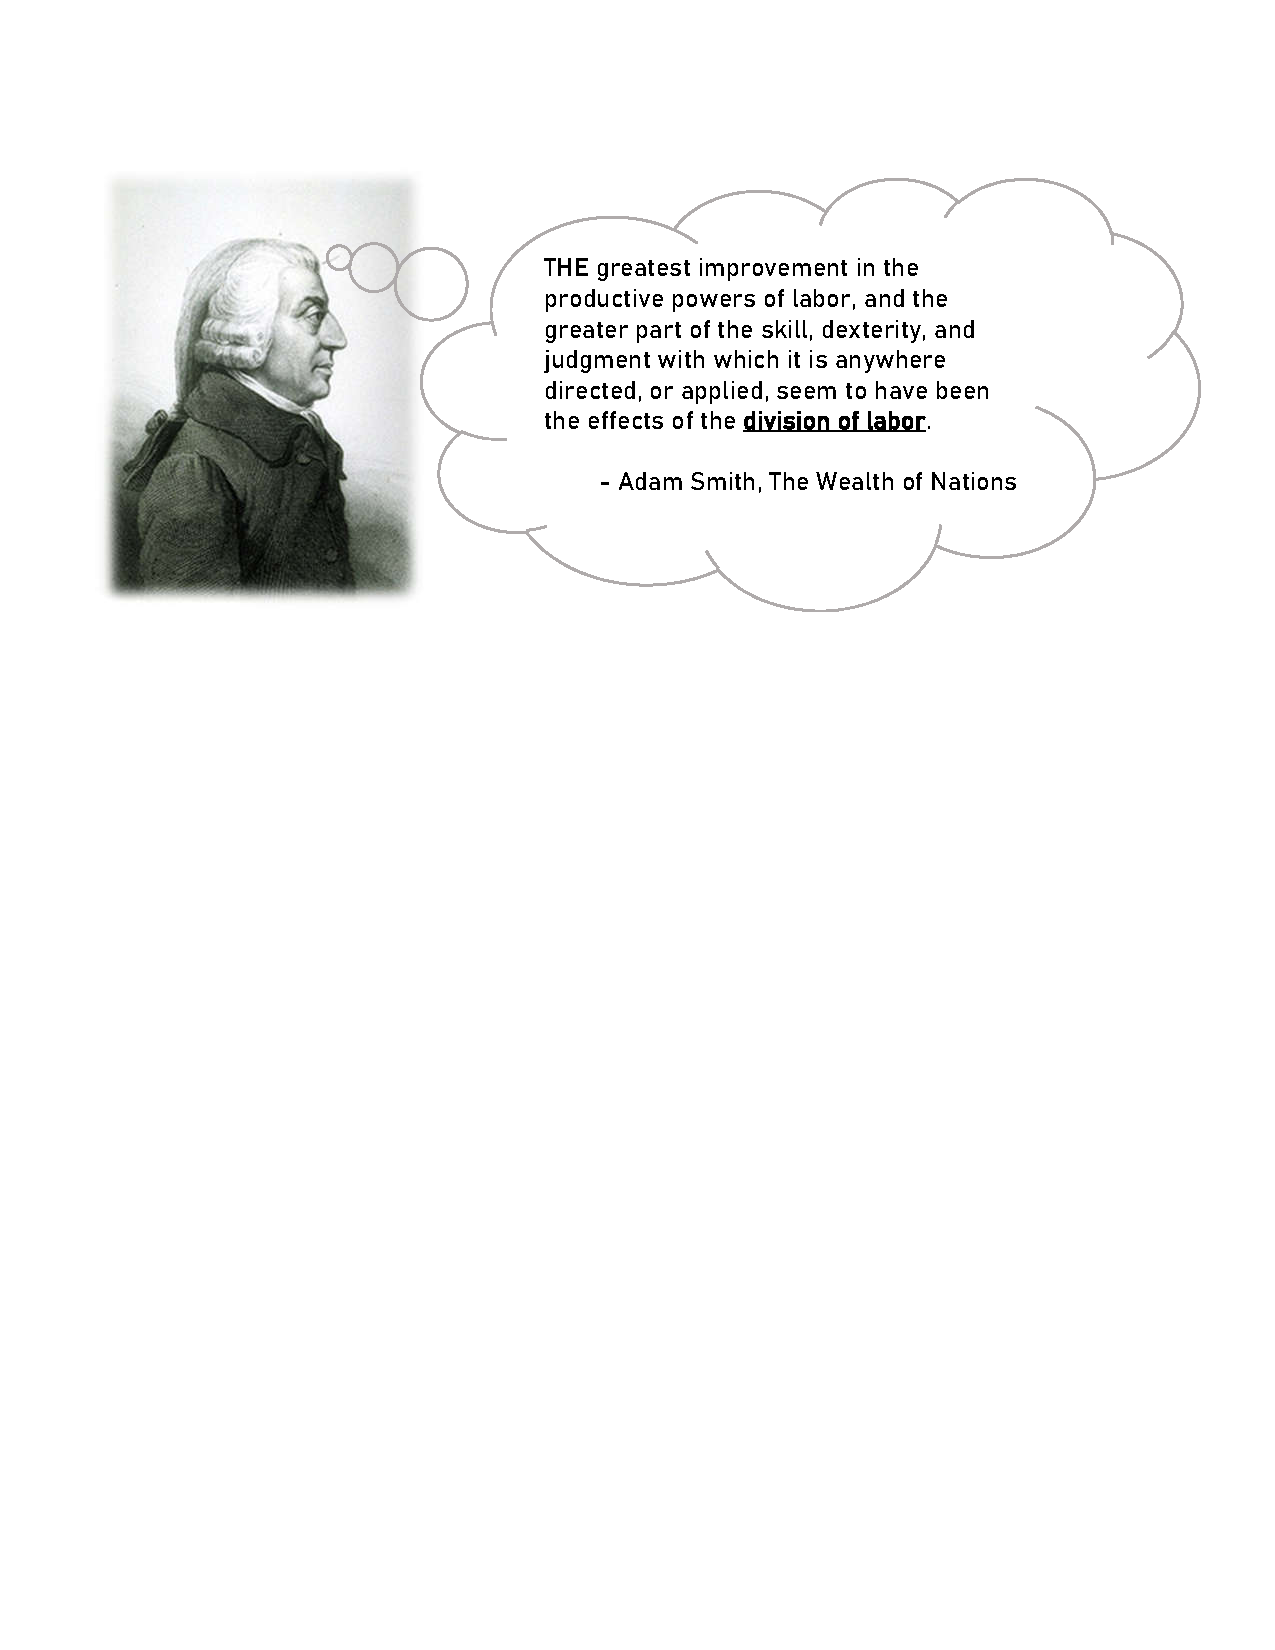
\includegraphics[width=0.90\textwidth]{material/crop-adam-smith.pdf}\\

\end{frame}

%-------------------------------------------------------------------------------
%-------------------------------------------------------------------------------
\begin{frame}\frametitle{Partners}\vspace{1.0cm}

\begin{columns}[t]

\column{.5\textwidth}
\centering \\  \vspace{-1.25cm}
    % Institute for Numerical Simulation
	
\includegraphics[width=0.3\textwidth]{material/crop-cooperation-ins.png} \\\vspace{-0.5cm}
		\footnotesize{Institute for \\ Numerical Simulation}\vspace{0.3cm}   \\ \vspace{0.5cm}
	% DIW
	
\includegraphics[width=0.45\textwidth]{material/crop-cooperation-diw.png} \\ \vspace{0.5cm}
	% Statistics Norway
	
\includegraphics[width=0.55\textwidth]{material/crop-cooperation-ssb.png} \\

\column{.5\textwidth}
	\centering \\ \vspace{-0.5cm}
	% Smart Data Analytics
	
\includegraphics[width=0.575\textwidth]{material/crop-cooperation-sda.png} \\ \vspace{0.85cm}
	% LIMES
	
\includegraphics[width=0.425\textwidth]{material/crop-cooperation-limes.png} \\ \vspace{0.4cm}
	% Lausanne
 	
\includegraphics[width=0.4\textwidth]{material/crop-cooperation-lausanne.png} \\

\column{.5\textwidth}
\centering \\

\end{columns}

\end{frame}
%-------------------------------------------------------------------------------
%-------------------------------------------------------------------------------
\begin{frame}\frametitle{What we are doing}\vspace{0.25cm}

\alert{Economic models}
\vspace{0.3cm}
\begin{itemize}\setlength\itemsep{1em}
	\item \makebox[2.25cm][l]{\alert<1>{respy}}
                \only<1>{
                        \explanation{
												Finite-horizon discrete Markov decision problem\\
                                Labor economics
                        }
                }
	\item \makebox[2.25cm][l]{\alert<2>{ruspy}}
                \only<2>{
                        \explanation{
												Infinite-horizon discrete Markov decision problem\\
                                Industrial organization
                        }
                }

		\item \makebox[2.25cm][l]{\alert<3>{pydsge}}
										\only<3>{
														\explanation{
														Dynamic stochastic general equilibrium model\\
														Monetary economics
														}
										}

\end{itemize}

\end{frame}
%-------------------------------------------------------------------------------
%-------------------------------------------------------------------------------
\begin{frame}\frametitle{What we are doing}\vspace{0.25cm}

	\heading{Analysis pipeline}\vspace{0.3cm}

	\begin{itemize}\setlength\itemsep{1em}
	        \item \makebox[2.25cm][l]{\alert<1>{estimagic}}
	                \only<1>{
	                        \explanation{
													Numerical optimization \\
	                                Estimating structural econometric models
	                        }
	                }
					\item \makebox[2.25cm][l]{\alert<2>{econsa}}
	                \only<2>{
	                        \explanation{%
													Sensitivity analysis \\
																	Assessing uncertainty of model implications
																	                        }
	                }

									\item \makebox[2.25cm][l]{\alert<3>{robupy}}
					                \only<3>{
					                        \explanation{%
																	Robust optimization \\
																					Incorporating model ambiguity
																					                        }
					                }

	\end{itemize}

	\vspace{0.50cm}

\only<4>{
\hspace{0.3cm}$\Rightarrow$  Intellectual arbitrage from work in applied mathematics\\\vspace{1em}
}
\only<5>{
	\hspace{0.3cm}$\Rightarrow$  Intellectual arbitrage from work in applied mathematics\\\vspace{1em}
	\hspace{0.3cm}$\Rightarrow$ Adapted to the needs of economists
}
\end{frame}
%-------------------------------------------------------------------------------
%-------------------------------------------------------------------------------
\begin{frame}\frametitle{Development}

	\begin{multicols}{2}
	\heading{Workflow}\vspace{0.3cm}
	\begin{itemize}\setlength\itemsep{1em}
	\item GitHub organization
	\item Code reviews
	\item Testing harness
	\item Continuous integration
	\end{itemize}

\columnbreak
	\pause

  \heading{Support}\vspace{0.3cm}
	\begin{itemize}\setlength\itemsep{1em}
	\item Documentation
	\item Chatroom
	\item Hackathon
	\item Conferences
	\end{itemize}
	\end{multicols}

\end{frame}
%-------------------------------------------------------------------------------
%-------------------------------------------------------------------------------
